\section{File Systems}

\subsection{File abstraction}
A \textcolor{Blue}{\textbf{file}} is a named sequence of bytes. \textcolor{Bittersweet}{Metadata}: name, type, size, owner, permissions, timestamps (atime, mtime, ctime), block pointers.
Operations: \texttt{open}, \texttt{read}, \texttt{write}, \texttt{close}, \texttt{lseek}, \texttt{stat}, \texttt{unlink}.

\paragraph{Key syscalls}
\begin{itemize}
  \item \texttt{int \textcolor{Bittersweet}{open}(path, flags, mode)}: returns FD. Flags: \texttt{O\_RDONLY}, \texttt{O\_WRONLY}, \texttt{O\_RDWR}, \texttt{O\_CREAT}, \texttt{O\_APPEND}, \texttt{O\_TRUNC}.
  \item \texttt{ssize\_t \textcolor{Bittersweet}{read}(fd,buf,n)} / \texttt{\textcolor{Bittersweet}{write}(fd,buf,n)}: advance file offset.
  \item \texttt{off\_t \textcolor{Bittersweet}{lseek}(fd,off,whence)}: \texttt{SEEK\_SET}, \texttt{SEEK\_CUR}, \texttt{SEEK\_END}.
  \item \texttt{int \textcolor{Bittersweet}{close}(fd)}, \texttt{int \textcolor{Bittersweet}{unlink}(path)}, \texttt{int \textcolor{Bittersweet}{stat}(path,\&buf)}.
\end{itemize}

\paragraph{Three-level FD indirection}
\textcolor{Bittersweet}{Per-process FD table} (in PCB; FDs 0/1/2 = stdin/out/err) $\to$ \textcolor{Bittersweet}{system-wide open-file table} (per-open offset, mode, ref count) $\to$ \textcolor{Bittersweet}{in-memory inode table}. Multiple opens of one file share an inode but get separate offsets; \texttt{dup}/\texttt{fork} share an open-file-table entry (and thus the offset).
\textcolor{Bittersweet}{OFT ref count} $=$ \#FDs pointing at the entry; \texttt{fork} increments by \#parent FDs (each child FD shares); \texttt{close(fd)} decrements; entry freed at 0.

\subsection{Directory structures}
\begin{itemize}
  \item \textcolor{Bittersweet}{Single-level}: one flat namespace; name collisions.
  \item \textcolor{Bittersweet}{Two-level}: per-user directory; isolated namespaces.
  \item \textcolor{Bittersweet}{Tree}: hierarchical; absolute (\texttt{/a/b}) vs relative (\texttt{./b}, \texttt{../b}); \texttt{.} and \texttt{..}.
  \item \textcolor{Bittersweet}{Acyclic graph}: hard/symbolic links; multiple paths to one inode.
\end{itemize}

\paragraph{Hard vs symbolic links}
\begin{tabular}{@{}lcc@{}}
\toprule
property & hard & symlink \\
\midrule
indirection & 0 (extra dirent) & extra inode \\
cross-FS & no & yes \\
can dangle & no & yes \\
target dirs & no (cycle risk) & yes \\
inc \texttt{nlink} & yes & no \\
\bottomrule
\end{tabular}

\subsection{File-system mount}
\texttt{mount} attaches a FS at a directory; subsequent path resolution redirects at the mount point. Multiple FSes share one namespace.

\subsection{Block allocation}
\paragraph{Contiguous} All blocks consecutive.
\textcolor{ForestGreen}{+}: simple, fastest seek, random access via $(\text{start}+i)$.
\textcolor{Bittersweet}{$-$}: external fragmentation; growth requires relocation.

\paragraph{Linked list} Each block stores a next-pointer.
\textcolor{ForestGreen}{+}: no external frag; trivial growth.
\textcolor{Bittersweet}{$-$}: random access is O($n$); pointer overhead inside data block; one corrupt link loses the rest.

\paragraph{FAT} A separate \textcolor{Blue}{File Allocation Table} entry per disk block; the file's chain lives in the FAT, not the data blocks.
\textcolor{ForestGreen}{+}: random access via in-memory FAT; no in-block pointers.
\textcolor{Bittersweet}{$-$}: FAT is normally cached in RAM for fast random access; large volumes make this expensive. FAT corruption is catastrophic. Variants \textcolor{ForestGreen}{FAT12/16/32} differ in entry width.

\paragraph{Indexed (inode)} Per-file index block lists data-block pointers.
\textcolor{ForestGreen}{+}: fast random access; no external frag.
\textcolor{Bittersweet}{$-$}: index-block overhead per file.

\paragraph{Multi-level inode (\textcolor{ForestGreen}{Unix ext2})}
Inode holds 12 \textcolor{Bittersweet}{direct} ptrs $+$ 1 \textcolor{Bittersweet}{single-} $+$ 1 \textcolor{Bittersweet}{double-} $+$ 1 \textcolor{Bittersweet}{triple-indirect}.

\begin{center}
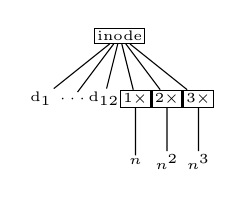
\begin{tikzpicture}[every node/.style={font=\tiny,inner sep=1pt},level distance=8mm,sibling distance=4mm]
\node[draw,rectangle] (i) {inode}
  child {node {d$_1$}}
  child {node {$\cdots$}}
  child {node {d$_{12}$}}
  child {node[draw] (s) {1$\times$} child {node {$n$}}}
  child {node[draw] (d) {2$\times$} child {node {$n^2$}}}
  child {node[draw] (t) {3$\times$} child {node {$n^3$}}};
\end{tikzpicture}
\end{center}

\noindent\begin{tabular}{@{}ll@{}}
\toprule
region & max file size ($B{=}4$KB, $s{=}4$B, $n{=}1024$) \\
\midrule
direct only & $\le 48$ KB \\
$+$ single & $\le 4$ MB$+48$ KB \\
$+$ double & $\le 4$ GB \\
$+$ triple & $\le 4$ TB \\
\bottomrule
\end{tabular}

\textcolor{Bittersweet}{Real-ext2 cap}: 32-bit \texttt{i\_size} bounds files at $\approx 2$ TB regardless of fanout.

\subsection{Free-space management}
\begin{itemize}
  \item \textcolor{Bittersweet}{Bitmap}: 1 bit per block; compact ($n$ blocks $\to n/8$ bytes); fast bit-scan finds free runs.
  \item \textcolor{Bittersweet}{Linked list}: next-free-block pointer chain through free blocks; slow scan.
  \item \textcolor{Bittersweet}{Grouping}: a block holds pointers to next $N$ free blocks plus a pointer to the next group block.
  \item \textcolor{Bittersweet}{Counting}: store (start, length) extents; compact when free regions are large.
\end{itemize}

\subsection{Buffer cache}
RAM cache of disk blocks. Reads check cache first; writes mark blocks dirty (\textcolor{Bittersweet}{write-back}); a daemon flushes periodically; \texttt{sync}/\texttt{fsync}/\texttt{fdatasync} forces flush. Trades durability for throughput.

\paragraph{Directory implementation}
\textcolor{Bittersweet}{Linear list} (simple, $O(n)$ search), \textcolor{Bittersweet}{hash table} ($O(1)$ avg, collisions), \textcolor{Bittersweet}{B-tree} ($O(\log n)$).

\subsection{Case studies}
\paragraph{FAT} Boot sector $\to$ FAT1 $\to$ FAT2 (mirror) $\to$ root dir (fixed-size on FAT12/16) $\to$ data area. Directory entry: 8.3 name, attrs, first cluster, size. Cluster-level allocation unit.
\paragraph{FAT sizing} Max blocks $=2^w$ where $w$ = usable entry-width bits (FAT16 reserves a few; usable $\approx 2^{16}-$ reserved). Max partition $=$ max-blocks $\times$ cluster size. Min pointer width $=\lceil\log_2(\text{total blocks})\rceil$ rounded up to bytes. \textcolor{Bittersweet}{On-demand FAT}: keep one FAT block resident; access to a non-resident entry costs $+1$ disk read.
\paragraph{ext2} Disk split into \textcolor{Bittersweet}{block groups}, each with \textcolor{Bittersweet}{superblock} (magic \texttt{0xEF53}, block/inode counts) (replicated), \textcolor{Bittersweet}{group descriptor table}, \textcolor{Bittersweet}{block bitmap}, \textcolor{Bittersweet}{inode bitmap}, \textcolor{Bittersweet}{inode table}, data blocks. 128-byte inode with 12+1+1+1 pointer scheme. Per-group locality reduces seeks.
\paragraph{Crash recovery}
\textcolor{Bittersweet}{fsck}: full-disk scan of bitmaps, inodes, directory hierarchy, link counts; slow on big disks.
\textcolor{Bittersweet}{Journaling} (ext3+, NTFS): write-ahead log of metadata changes commits atomically; replay on crash; fast recovery.

\subsection{Disk scheduling}
The disk arm has measurable seek time; the OS reorders pending I/O to reduce it.
\begin{itemize}
  \item \textcolor{Bittersweet}{FCFS}: serve in arrival order. Fair, simple; poor seek locality.
  \item \textcolor{Bittersweet}{SSTF} (shortest-seek-time-first): pick the request closest to the current head. Lower mean seek; risk of \textcolor{Bittersweet}{starvation} for distant requests.
  \item \textcolor{Bittersweet}{SCAN} (elevator): head sweeps end-to-end servicing requests in passing, then reverses.
  \item \textcolor{Bittersweet}{C-SCAN}: like SCAN but on reaching the end, jump back without serving in reverse — more uniform wait times.
  \item \textcolor{Bittersweet}{LOOK / C-LOOK}: as SCAN/C-SCAN but reverse at the last pending request, not the disk edge.
\end{itemize}
\textcolor{ForestGreen}{File protection} (Unix): \texttt{rwx} bits per owner/group/other (e.g., \texttt{0755}); \texttt{setuid} runs with the file owner's UID; \texttt{setgid} runs with the file's group GID; \texttt{sticky} bit on shared dirs (\texttt{/tmp}) restricts deletion to the file's owner.

\paragraph{File types (Unix)}
\textcolor{Bittersweet}{Regular} (data), \textcolor{Bittersweet}{directory}, \textcolor{Bittersweet}{symlink}, \textcolor{Bittersweet}{character device} (unbuffered, byte-stream — tty, \texttt{/dev/null}), \textcolor{Bittersweet}{block device} (buffered, sector — disks), \textcolor{Bittersweet}{FIFO} (named pipe), \textcolor{Bittersweet}{socket}.

\paragraph{Timestamps}
\textcolor{Bittersweet}{atime} (last access — costly to update on every read; many systems use \texttt{noatime}), \textcolor{Bittersweet}{mtime} (last data write), \textcolor{Bittersweet}{ctime} (last inode/metadata change).

\paragraph{Sparse files}
A write past current EOF leaves a \textcolor{Bittersweet}{hole}; no blocks allocated for the gap; reads return zeros. Saves space for large but mostly-empty files (databases, virtual disks). \texttt{fallocate} explicitly allocates / punches holes.

\paragraph{Pathname resolution}
Absolute (\texttt{/a/b/c}) starts at root inode; relative starts at CWD inode. For each component: read containing dir's inode, check execute permission, look up name, fetch target inode. Symlinks restart resolution at the target path (cycle detection needed). The kernel maintains a \textcolor{Bittersweet}{dentry / DNLC} (directory-entry / name-lookup cache) to avoid repeated disk reads.

\paragraph{Permissions (octal)}
Three triples (owner, group, other) of \texttt{rwx}. Octal: $r=4$, $w=2$, $x=1$.
\textcolor{ForestGreen}{0755} = \texttt{rwxr-xr-x} (typical executable); \textcolor{ForestGreen}{0644} = \texttt{rw-r--r--} (typical file); \textcolor{ForestGreen}{0700} = \texttt{rwx------} (private dir).

\textcolor{Bittersweet}{umask}: default mode of new files = \texttt{mode \& \textasciitilde umask}; common \texttt{umask}=\texttt{022}.

\paragraph{Disk-scheduling example}
Track 0..199, head at 53, queue \texttt{98 183 37 122 14 124 65 67}.
\begin{itemize}
  \item \textcolor{Bittersweet}{FCFS}: total head movement $= |53\!-\!98|+|98\!-\!183|+\dots = 640$.
  \item \textcolor{Bittersweet}{SSTF}: pick nearest each time $\Rightarrow$ 65,67,37,14,98,122,124,183; movement $\approx 236$.
  \item \textcolor{Bittersweet}{LOOK} (toward 0 first): 37,14,65,67,98,122,124,183; $\approx$ 208.
  \item \textcolor{ForestGreen}{C-SCAN} (toward 199, jump to 0): 65,67,98,122,124,183,(199),(0),14,37; $\approx 382$.
  \item \textcolor{ForestGreen}{C-LOOK} (toward 183, jump to 14): 65,67,98,122,124,183,14,37; $\approx 322$.
\end{itemize}

\paragraph{Block size trade-off}
\textcolor{Bittersweet}{Block size}: large = fewer ptrs / better seq throughput / more internal frag; small = opposite.

\paragraph{ext2 directory entry}
Variable length record per file:
\begin{itemize}
  \item \texttt{inode\_no} (4 B), \texttt{rec\_len} (2 B), \texttt{name\_len} (1 B), \texttt{file\_type} (1 B), then up-to-255-byte name.
  \item Deleted entries are coalesced into the previous entry's \texttt{rec\_len} (form a hole) — fast unlink, slower lookup.
\end{itemize}

\paragraph{Journaling modes}
\textcolor{Bittersweet}{writeback} (metadata journaled only; data may be inconsistent on crash); \textcolor{Bittersweet}{ordered} (default in ext3; journal metadata, write data before metadata commit); \textcolor{Bittersweet}{full} (journal both data and metadata; safest, slowest).

